%%%%%%%%%%%%%%%%%%%%%%%%%%%%%%%%%%%%%%%%%
% Beamer Presentation
% LaTeX Template
% Version 1.0 (10/11/12)
%
% This template has been downloaded from:
% http://www.LaTeXTemplates.com
%
% License:
% CC BY-NC-SA 3.0 (http://creativecommons.org/licenses/by-nc-sa/3.0/)
%
%%%%%%%%%%%%%%%%%%%%%%%%%%%%%%%%%%%%%%%%%

%----------------------------------------------------------------------------------------
%	PACKAGES AND THEMES
%----------------------------------------------------------------------------------------

\documentclass[UTF8,aspectratio=169,14pt]{ctexbeamer}

\usepackage{hyperref}
\hypersetup{
	colorlinks=true,
	linkcolor=red,
	anchorcolor=blue,
	citecolor=green
}

\mode<presentation> {
	
	% The Beamer class comes with a number of default slide themes
	% which change the colors and layouts of slides. Below this is a list
	% of all the themes, uncomment each in turn to see what they look like.
	
	%\usetheme{default}
	%\usetheme{AnnArbor}
	%\usetheme{Antibes}
	%\usetheme{Bergen}
	%\usetheme{Berkeley}
	%\usetheme{Berlin}
	%\usetheme{Boadilla}
	%\usetheme{CambridgeUS}
	%\usetheme{Copenhagen}
	%\usetheme{Darmstadt}
	%\usetheme{Dresden}
	%\usetheme{Frankfurt}
	%\usetheme{Goettingen}
	%\usetheme{Hannover}
	%\usetheme{Ilmenau}
	%\usetheme{JuanLesPins}
	%\usetheme{Luebeck}
	\usetheme{Madrid}
	%\usetheme{Malmoe}
	%\usetheme{Marburg}
	%\usetheme{Montpellier}
	%\usetheme{PaloAlto}
	%\usetheme{Pittsburgh}
	%\usetheme{Rochester}
	%\usetheme{Singapore}
	%\usetheme{Szeged}
	%\usetheme{Warsaw}
	
	% As well as themes, the Beamer class has a number of color themes
	% for any slide theme. Uncomment each of these in turn to see how it
	% changes the colors of your current slide theme.
	
	%\usecolortheme{albatross}
	%\usecolortheme{beaver}
	%\usecolortheme{beetle}
	%\usecolortheme{crane}
	%\usecolortheme{dolphin}
	%\usecolortheme{dove}
	%\usecolortheme{fly}
	%\usecolortheme{lily}
	%\usecolortheme{orchid}
	%\usecolortheme{rose}
	%\usecolortheme{seagull}
	%\usecolortheme{seahorse}
	%\usecolortheme{whale}
	%\usecolortheme{wolverine}
	
	%\setbeamertemplate{footline} % To remove the footer line in all slides uncomment this line
	%\setbeamertemplate{footline}[page number] % To replace the footer line in all slides with a simple slide count uncomment this line
	
	%\setbeamertemplate{navigation symbols}{} % To remove the navigation symbols from the bottom of all slides uncomment this line
}

\usepackage{graphicx} % Allows including images
\graphicspath{{./figs/}}
\usepackage{booktabs} % Allows the use of \toprule, \midrule and \bottomrule in tables
\usepackage{longtable}
\usepackage{listings}
\usepackage{xcolor}
\lstset{numbers=left, %设置行号位置
	numberstyle=\tiny, %设置行号大小
	keywordstyle=\color{blue}, %设置关键字颜色
	commentstyle=\color[cmyk]{1,0,1,0}, %设置注释颜色
	frame=single, %设置边框格式
	escapeinside=``, %逃逸字符(1左面的键),用于显示中文
	%breaklines, %自动折行
	extendedchars=false, %解决代码跨页时,章节标题,页眉等汉字不显示的问题
	xleftmargin=2em,xrightmargin=2em, aboveskip=1em, %设置边距
	tabsize=4, %设置tab空格数
	showspaces=false %不显示空格
}
% Fonts
% \usepackage{libertine}
% \setmonofont{Courier}
\setCJKsansfont[ItalicFont=Noto Serif CJK SC Black, BoldFont=Noto Sans CJK SC Black]{Noto Sans CJK SC}


%----------------------------------------------------------------------------------------
%	TITLE PAGE
%----------------------------------------------------------------------------------------

\title[第1讲]{第12讲 :多处理器调度} % The short title appears at the bottom of every slide, the full title is only on the title page
\subtitle{第四节:CFS 调度}
\author{向勇、陈渝、李国良} % Your name
\institute[清华大学] % Your institution as it will appear on the bottom of every slide, may be shorthand to save space
{
	清华大学计算机系 \\ % Your institution for the title page
	\medskip
	\textit{xyong,yuchen,liguoliang@tsinghua.edu.cn} % Your email address
}
\date{\today} % Date, can be changed to a custom date


\begin{document}

\begin{frame}
\titlepage % Print the title page as the first slide
\end{frame}

%\begin{frame}
%\frametitle{提纲} % Table of contents slide, comment this block out to remove it
%\tableofcontents % Throughout your presentation, if you choose to use \section{} and \subsection{} commands, these will automatically be printed on this slide as an overview of your presentation
%\end{frame}
%
%%----------------------------------------------------------------------------------------
%%	PRESENTATION SLIDES\begin{itemize}
%%----------------------------------------------------------------------------------------
%
%%------------------------------------------------
%\section{第一节:课程概述} % Sections can be created in order to organize your presentation into discrete blocks, all sections and subsections are automatically printed in the table of contents as an overview of the talk
%%------------------------------------------------

% 从几个问题开始理解CFS调度器 http://linuxperf.com/?p=42
%http://repo-ck.com/bench/cpu_schedulers_compared.pdf
%红黑树虽然本质上是一棵二叉查找树,但它在二叉查找树的基础上增加了着色和相关的性质使得红黑树相对平衡,从而保证了红黑树的查找、插入、删除的时间复杂度最坏为O(log n)。
\begin{frame}
	\frametitle{CFS调度}
	\begin{columns}
	\begin{column}{.4\textwidth}
	\Large \centering
	
    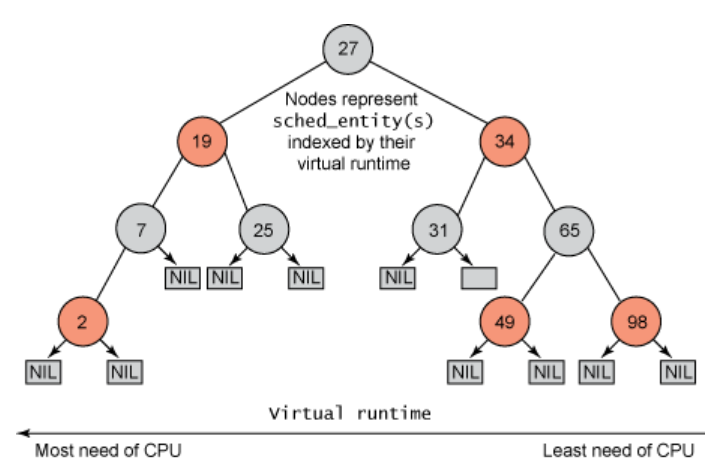
\includegraphics[width=1.\textwidth]{rbtree}
	
	\end{column}
	
	\begin{column}{.6\textwidth}
%		\large
\begin{itemize}
	\item 以前的Linux调度算法根据进程的优先级进行调度,即通过一系列运行指标确定进程的优先级,然后根据进程的优先级确定调度哪个进程
	\item CFS则转换了一种思路,它不计算优先级,而是通过计算进程消耗的CPU时间(标准化以后的虚拟CPU时间)来确定谁来调度。从而到达所谓的公平性。

	\end{itemize}

	\end{column}
\end{columns}
\end{frame}


%----------------------------------------------
\begin{frame}
	\frametitle{CFS调度}
	\begin{columns}
		\begin{column}{.4\textwidth}
			\Large \centering
			
			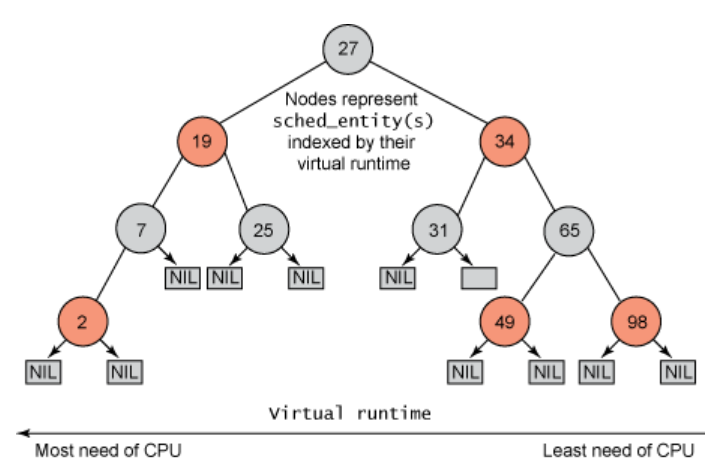
\includegraphics[width=1.\textwidth]{rbtree}
			
		\end{column}
		
		\begin{column}{.6\textwidth}
			绝对公平性:
			\begin{itemize}
				\item 把CPU当做一种资源,并记录下每一个进程对该资源使用的情况,在调度时,调度器总是选择消耗资源最少的进程来运行。
				\item 但这种绝对的公平有时也是一种不公平,因为有些进程的工作比其他进程更重要,我们希望能按照权重来分配CPU资源。
				
			\end{itemize}
			
		\end{column}
	\end{columns}
\end{frame}


%----------------------------------------------
\begin{frame}
	\frametitle{CFS调度}
	\begin{columns}
		\begin{column}{.4\textwidth}
			\Large \centering
			
			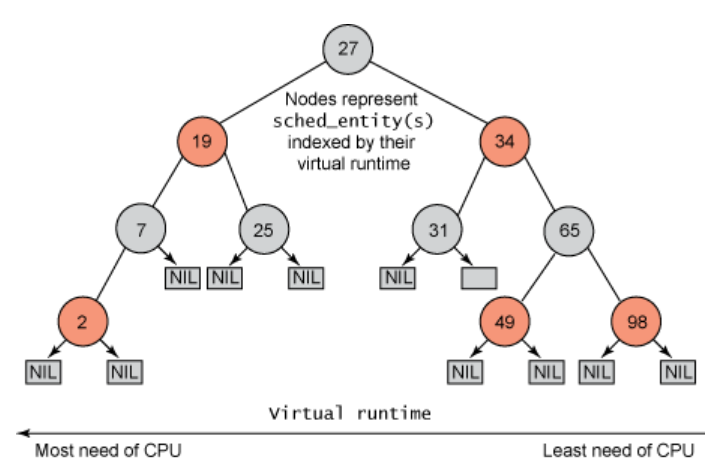
\includegraphics[width=1.\textwidth]{rbtree}
			
		\end{column}
	
		
		\begin{column}{.6\textwidth}
%			绝对公平性: \\
			相对公平性:
			\begin{itemize}
				\item 为了区别不同优先级的进程,就是会根据各个进程的权重分配运行时间
				\item 分配给进程的运行时间 = 调度周期 * 进程权重 / 所有进程权重之和
				\item 调度周期:将所处于TASK\_RUNNING态进程都调度一遍的时间
				
			\end{itemize}
			
		\end{column}
	\end{columns}
\end{frame}


%----------------------------------------------
\begin{frame}
	\frametitle{CFS调度}
	\begin{columns}
		\begin{column}{.4\textwidth}
			\Large \centering
			
			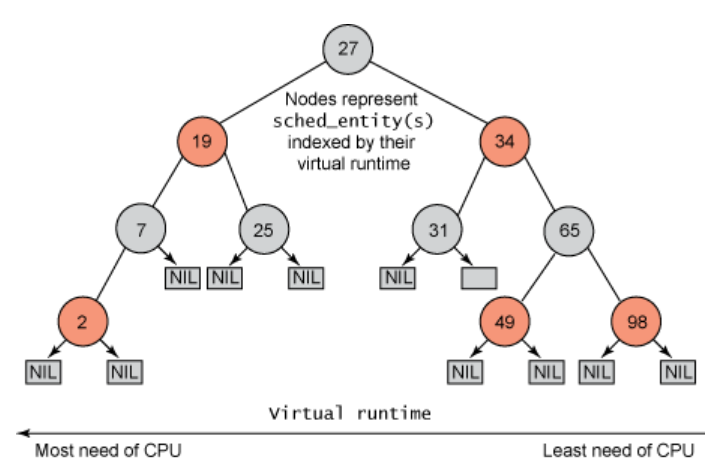
\includegraphics[width=1.\textwidth]{rbtree}
			
		\end{column}
		
		\begin{column}{.6\textwidth}
			%			绝对公平性: \\
			相对公平性:
			\begin{itemize}
				\item 比如系统中只两个进程A, B,权重分别为1和2,假设调度周期设为30ms,
				\item A的CPU时间为:30ms * (1/(1+2)) = 10ms
				\item B的CPU时间为:30ms * (2/(1+2)) = 20ms
				\item 在这30ms中A将运行10ms,B将运行20ms
				
			\end{itemize}
			
		\end{column}
	\end{columns}
\end{frame}



%----------------------------------------------
\begin{frame}
	\frametitle{CFS调度}
	\begin{columns}
		\begin{column}{.4\textwidth}
			\Large \centering
			
			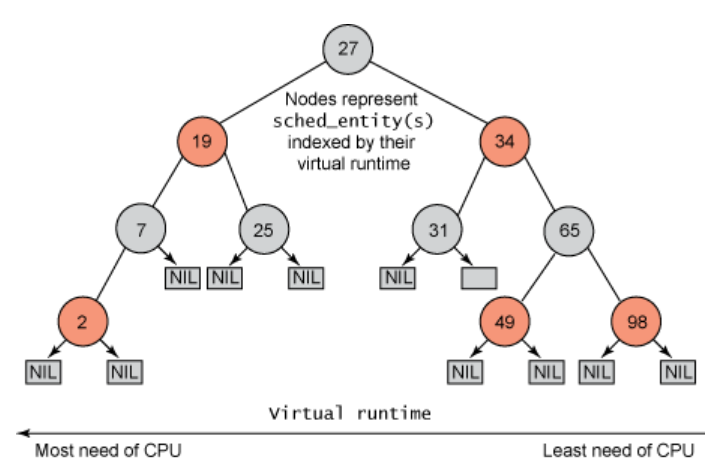
\includegraphics[width=1.\textwidth]{rbtree}
			
		\end{column}
		
		\begin{column}{.6\textwidth}
			%			绝对公平性: \\
			实现原理 \\
			Linux通过引入virtual runtime(vruntime)
			\begin{itemize}
				\item vruntime = 实际运行时间 * 1024 / 进程权重 
				\item 谁的vruntime值较小就说明它以前占用cpu的时间较短,受到了“不公平”对待,因此下一个运行进程就是它
				\item 这样既能公平选择进程,又能保证高优先级进程获得较多的运行时间。
			\end{itemize}
			
		\end{column}
	\end{columns}
\end{frame}


%----------------------------------------------
\begin{frame}
	\frametitle{CFS调度}
	\begin{columns}
		\begin{column}{.4\textwidth}
			\Large \centering
			
			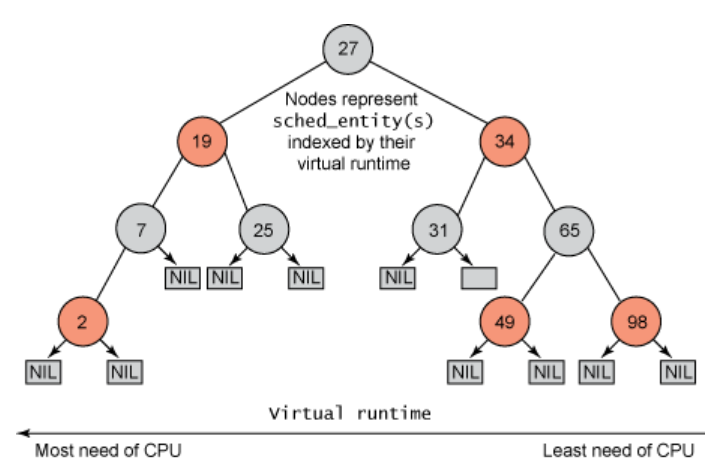
\includegraphics[width=1.\textwidth]{rbtree}
			
		\end{column}
		
		\begin{column}{.6\textwidth}
			%			绝对公平性: \\
			具体实现 
			\begin{itemize}
				\item Linux采用了一颗红黑树(对于多核调度,实际上每一个核有一个自己的红黑树),记录下每一个进程的vruntime
				\item 需要调度时,从红黑树中选取一个vruntime最小的进程出来运行
			\end{itemize}
			
		\end{column}
	\end{columns}
\end{frame}


%----------------------------------------------
\begin{frame}
	\frametitle{CFS调度}
	\begin{columns}
		\begin{column}{.4\textwidth}
			\Large \centering
			
			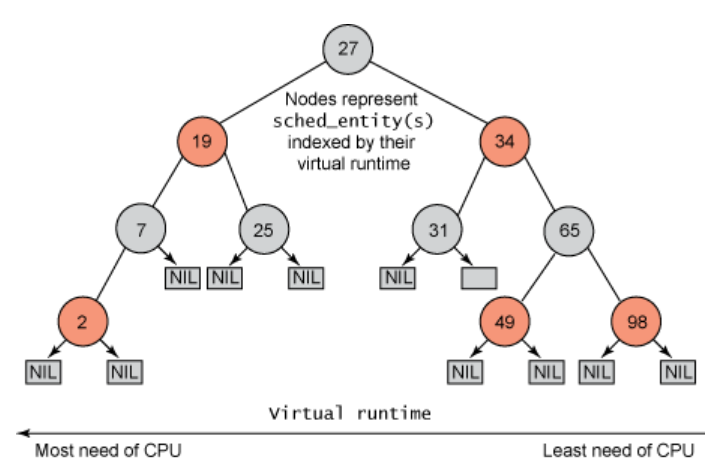
\includegraphics[width=.8\textwidth]{rbtree}

		\end{column}
		
		\begin{column}{.6\textwidth}

			具体实现 :权重如何决定?
			\begin{itemize}
				\item 权重由nice值确定,权重跟进程nice值之间有一一对应的关系
				\item 通过全局数组prio\_to\_weight来转换,nice值越大,权重越低。

			\end{itemize}
						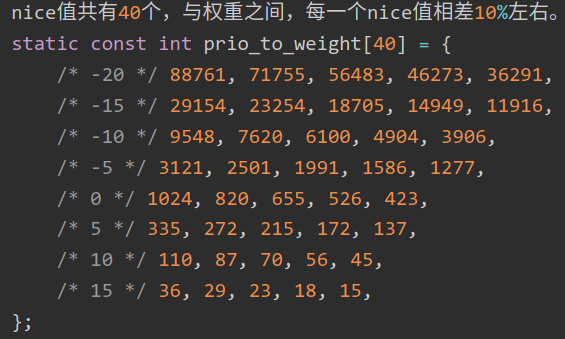
\includegraphics[width=.8\textwidth]{prio-to-weight}
		\end{column}
	\end{columns}
\end{frame}




%----------------------------------------------
\begin{frame}
	\frametitle{CFS调度}
	\begin{columns}
		\begin{column}{.4\textwidth}
			\Large \centering
			
			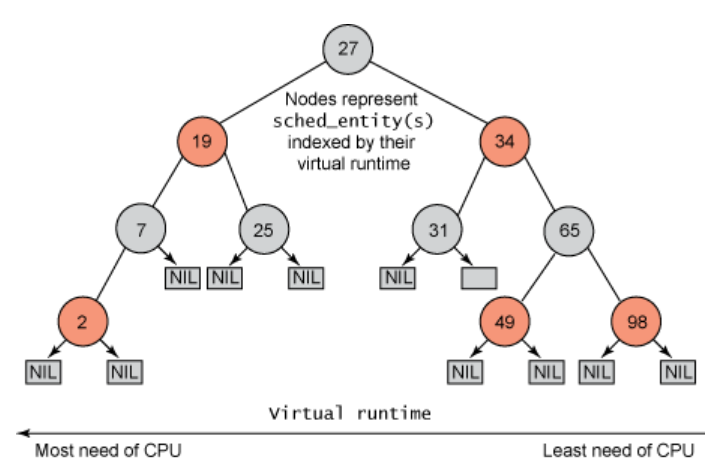
\includegraphics[width=.8\textwidth]{rbtree}
			
		\end{column}
		
		\begin{column}{.6\textwidth}
			
			具体实现 :新创建进程的vruntime是多少?
			\begin{itemize}
				\item 假如新进程的vruntime初值为0的话,比老进程的值小很多,那么它在相当长的时间内都会保持抢占CPU的优势,老进程就要饿死了,这显然是不公平的。
				\item 每个CPU的运行队列cfs\_rq都维护一个min\_vruntime字段,记录该运行队列中所有进程的vruntime最小值,新进程的初始vruntime值就以它所在运行队列的min\_vruntime为基础来设置,与老进程保持在合理的差距范围内。
			\end{itemize}
		\end{column}
	\end{columns}
\end{frame}


%----------------------------------------------
\begin{frame}
	\frametitle{CFS调度}
	\begin{columns}
		\begin{column}{.4\textwidth}
			\Large \centering
			
			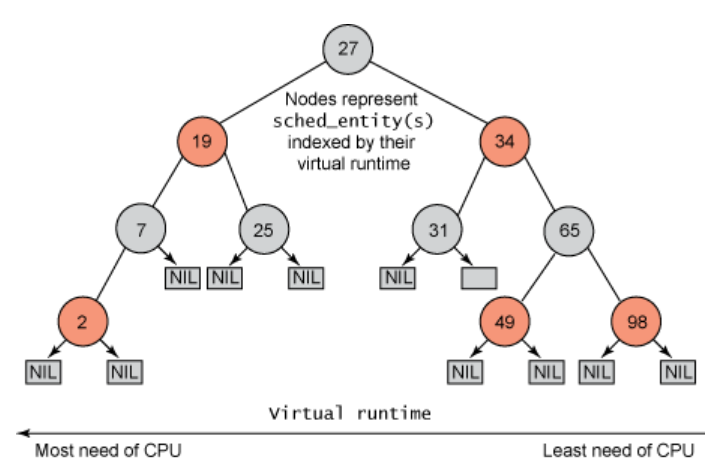
\includegraphics[width=.8\textwidth]{rbtree}
			
		\end{column}
		
		\begin{column}{.6\textwidth}
			
			具体实现 :休眠进程的vruntime一直保持不变吗?
			\begin{itemize}
				\item 如果休眠进程的 vruntime 保持不变,而其他运行进程的 vruntime 一直在推进,那么等到休眠进程终于唤醒的时候,它的vruntime比别人小很多,会使它获得长时间抢占CPU的优势,其他进程就要饿死了。

				\item 在休眠进程被唤醒时重新设置vruntime值,以min\_vruntime值为基础,给予一定的补偿,但不能补偿太多。
			\end{itemize}
		\end{column}
	\end{columns}
\end{frame}


%----------------------------------------------
\begin{frame}
	\frametitle{CFS调度}
	\begin{columns}
		\begin{column}{.4\textwidth}
			\Large \centering
			
			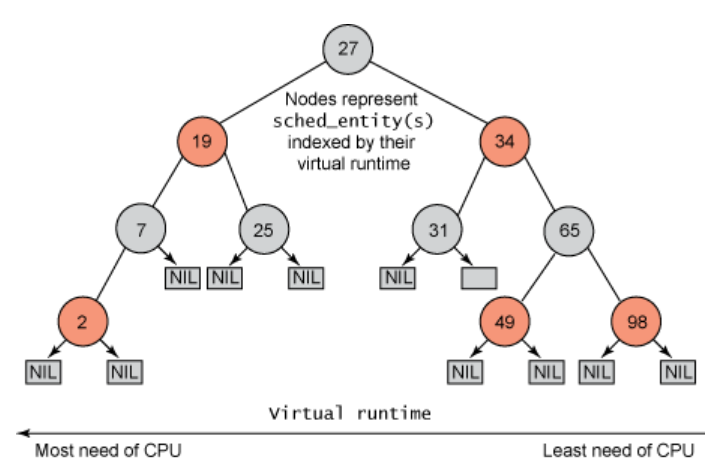
\includegraphics[width=.8\textwidth]{rbtree}
			
		\end{column}
		
		\begin{column}{.6\textwidth}
			
			具体实现 :休眠进程在唤醒时会立刻抢占CPU吗?
			\begin{itemize}
				\item 休眠进程在醒来的时候有能力抢占CPU是大概率事件,这也是CFS调度算法的本意,即保证交互式进程的响应速度,因为交互式进程等待用户输入会频繁休眠。
				
				\item 主动休眠的进程同样也会在唤醒时获得补偿,这类进程往往并不要求快速响应,它们同样也会在每次唤醒并抢占,这有可能会导致其它更重要的应用进程被抢占,有损整体性能。
				\item sched\_features的WAKEUP\_PREEMPT位
				
			\end{itemize}
		\end{column}
	\end{columns}
\end{frame}


%----------------------------------------------
\begin{frame}
	\frametitle{CFS调度}
	\begin{columns}
		\begin{column}{.4\textwidth}
			\Large \centering
			
			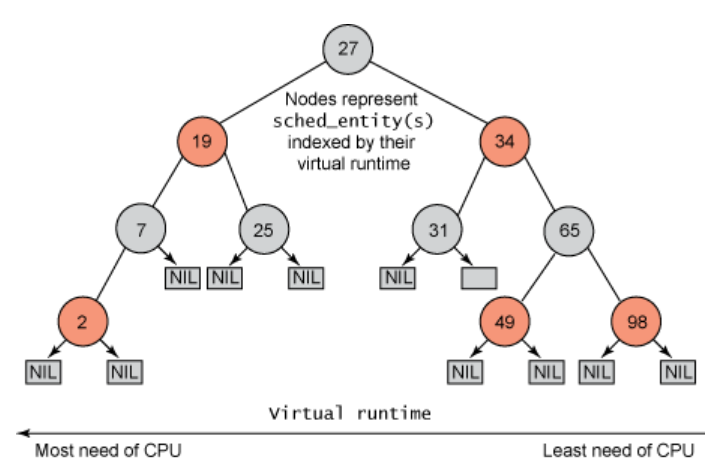
\includegraphics[width=.8\textwidth]{rbtree}
			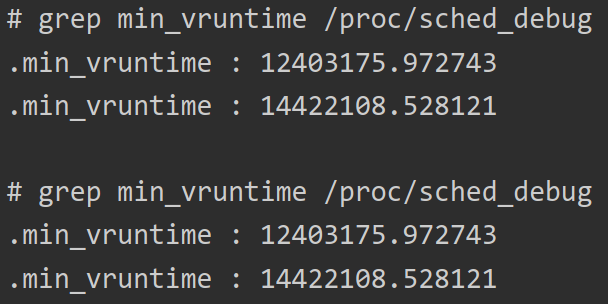
\includegraphics[width=1.\textwidth]{smp-min-vruntime}
		\end{column}
		
		\begin{column}{.6\textwidth}
			
			具体实现 :进程从一个CPU迁移到另一个CPU上的时候vruntime会不会变?
			\begin{itemize}
				\item 在多CPU的系统上,不同的CPU的负载不一样,有的CPU更忙一些,而每个CPU都有自己的运行队列,每个队列中的进程的vruntime也走得有快有慢,比如我们对比每个运行队列的min\_vruntime值,都会有不同
				\pause
				\item 当进程从一个CPU的运行队列中出来时, 它的vruntime要减去队列的min\_vruntime值;
				\item 当进程加入另一个CPU的运行队列时,它的vruntime要加上该队列的min\_vruntime值。
			\end{itemize}
			\centering
%			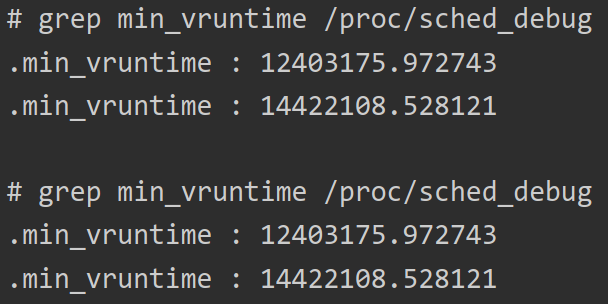
\includegraphics[width=.7\textwidth]{smp-min-vruntime}
		\end{column}
	\end{columns}
\end{frame}


%----------------------------------------------
\begin{frame}
	\frametitle{CFS调度}
	\begin{columns}
		\begin{column}{.4\textwidth}
			\Large \centering
			
			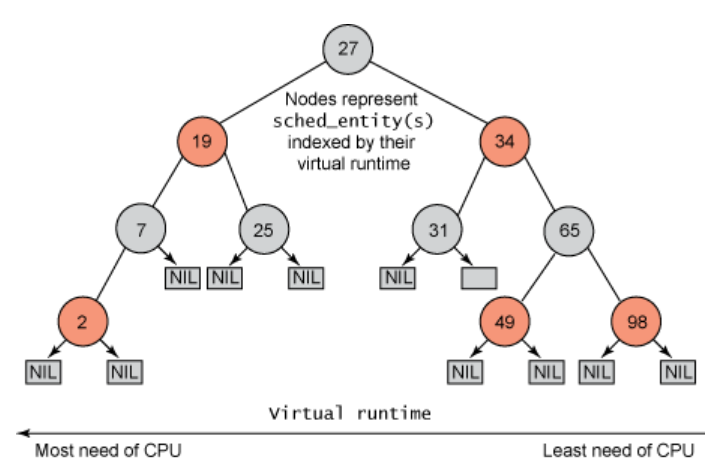
\includegraphics[width=.8\textwidth]{rbtree}
%			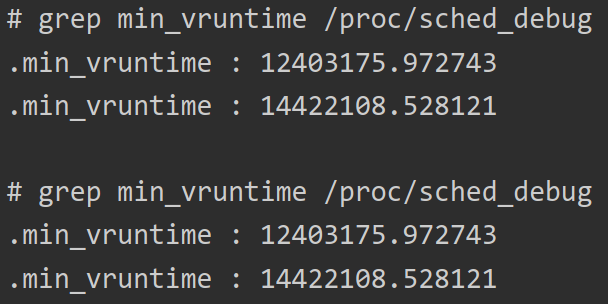
\includegraphics[width=1.\textwidth]{smp-min-vruntime}
		\end{column}
		
		\begin{column}{.6\textwidth}
			
			具体实现 :vruntime溢出问题
			\begin{itemize}
				\item 红黑树中实际的作为key的不是vruntime而是vruntime - min\_vruntime。min\_vruntime是当前红黑树中最小的key
				\item vruntime 的类型 usigned long
				\item 进程的虚拟时间是一个递增的正值,因此它不会是负 数,但是它有它的上限,就是unsigned long所能表示的最大值,如果溢出了,那么它就会从0开始回滚,如果这样的话,结果会怎样?
			\end{itemize}
			\centering

		\end{column}
	\end{columns}
\end{frame}


%----------------------------------------------
\begin{frame}
	\frametitle{CFS调度}
	\begin{columns}
		\begin{column}{.4\textwidth}
			\Large \centering
			
			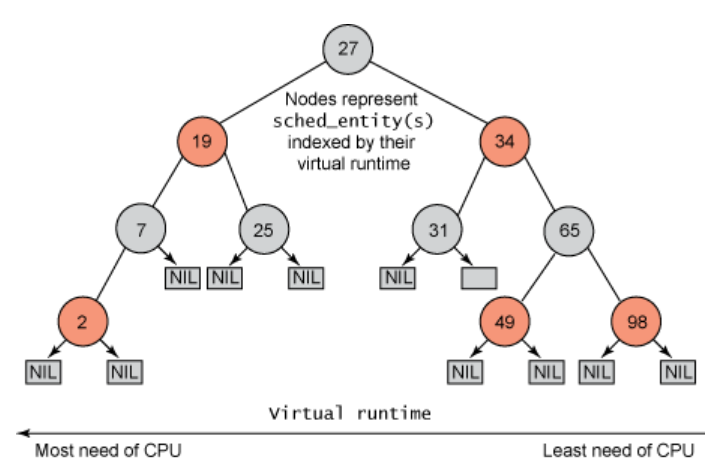
\includegraphics[width=.8\textwidth]{rbtree}
			%			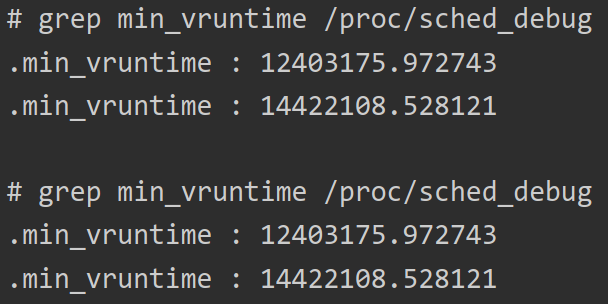
\includegraphics[width=1.\textwidth]{smp-min-vruntime}
		\end{column}
		
		\begin{column}{.6\textwidth}
			
			具体实现 :vruntime溢出问题
			
\begin{block}{一个例子}
unsigned char a = 251, b = 254;  \\
b += 5; \\
//b回滚了,导致a大于b,应该是b比a大8\\
 
//怎么做到真正的结果呢?改为以下:\\
unsigned char a = 251, b = 254;\\
b += 5; \\
signed char c = a - 250, d = b - 250; \\
//到此判断c和d的大小
\end{block}			

		\end{column}
	\end{columns}
\end{frame}
%----------------------------------------------
%----------------------------------------------
\end{document}
